\documentclass[journal,12pt,twocolumn]{IEEEtran}

\usepackage{setspace}
\usepackage{gensymb}
\singlespacing
\usepackage[cmex10]{amsmath}

\usepackage{amsthm}

\usepackage{mathrsfs}
\usepackage{txfonts}
\usepackage{stfloats}
\usepackage{bm}
\usepackage{cite}
\usepackage{cases}
\usepackage{subfig}
\usepackage{graphicx}
\usepackage{longtable}
\usepackage{multirow}

\usepackage{enumitem}
\usepackage{mathtools}
\usepackage{steinmetz}
\usepackage{tikz}
\usepackage{circuitikz}
\usepackage{verbatim}
\usepackage{tfrupee}
\usepackage[breaklinks=true]{hyperref}
\usepackage{graphicx}
\usepackage{tkz-euclide}

\usetikzlibrary{calc,math}
\usepackage{listings}
    \usepackage{color}                                            %%
    \usepackage{array}                                            %%
    \usepackage{longtable}                                        %%
    \usepackage{calc}                                             %%
    \usepackage{multirow}                                         %%
    \usepackage{hhline}                                           %%
    \usepackage{ifthen}                                           %%
    \usepackage{lscape}     
\usepackage{multicol}
\usepackage{chngcntr}

\DeclareMathOperator*{\Res}{Res}

\renewcommand\thesection{\arabic{section}}
\renewcommand\thesubsection{\thesection.\arabic{subsection}}
\renewcommand\thesubsubsection{\thesubsection.\arabic{subsubsection}}

\renewcommand\thesectiondis{\arabic{section}}
\renewcommand\thesubsectiondis{\thesectiondis.\arabic{subsection}}
\renewcommand\thesubsubsectiondis{\thesubsectiondis.\arabic{subsubsection}}


\hyphenation{op-tical net-works semi-conduc-tor}
\def\inputGnumericTable{}                                 %%

\lstset{
%language=C,
frame=single, 
breaklines=true,
columns=fullflexible
}
\begin{document}
\newtheorem{lemma}{Lemma}[section]
\newcommand{\BEQA}{\begin{eqnarray}}
\newcommand{\EEQA}{\end{eqnarray}}
\newcommand{\define}{\stackrel{\triangle}{=}}
\bibliographystyle{IEEEtran}
\raggedbottom
\setlength{\parindent}{0pt}
\providecommand{\mbf}{\mathbf}
\providecommand{\pr}[1]{\ensuremath{\Pr\left(#1\right)}}
\providecommand{\qfunc}[1]{\ensuremath{Q\left(#1\right)}}
\providecommand{\sbrak}[1]{\ensuremath{{}\left[#1\right]}}
\providecommand{\lsbrak}[1]{\ensuremath{{}\left[#1\right.}}
\providecommand{\rsbrak}[1]{\ensuremath{{}\left.#1\right]}}
\providecommand{\brak}[1]{\ensuremath{\left(#1\right)}}
\providecommand{\lbrak}[1]{\ensuremath{\left(#1\right.}}
\providecommand{\rbrak}[1]{\ensuremath{\left.#1\right)}}
\providecommand{\cbrak}[1]{\ensuremath{\left\{#1\right\}}}
\providecommand{\lcbrak}[1]{\ensuremath{\left\{#1\right.}}
\providecommand{\rcbrak}[1]{\ensuremath{\left.#1\right\}}}
\theoremstyle{remark}
\newtheorem{rem}{Remark}
\newcommand{\sgn}{\mathop{\mathrm{sgn}}}
\providecommand{\abs}[1]{\vert#1\vert}
\providecommand{\res}[1]{\Res\displaylimits_{#1}} 
\providecommand{\norm}[1]{\lVert#1\rVert}
\providecommand{\sinc}{sinc}
%\providecommand{\norm}[1]{\lVert#1\rVert}
\providecommand{\mtx}[1]{\mathbf{#1}}
\providecommand{\mean}[1]{E[ #1 ]}
\providecommand{\fourier}{\overset{\mathcal{F}}{ \rightleftharpoons}}
%\providecommand{\hilbert}{\overset{\mathcal{H}}{ \rightleftharpoons}}
\providecommand{\system}{\overset{\mathcal{H}}{ \longleftrightarrow}}
	%\newcommand{\solution}[2]{\textbf{Solution:}{#1}}
\newcommand{\solution}{\noindent \textbf{Solution: }}
\newcommand{\cosec}{\,\text{cosec}\,}
\providecommand{\dec}[2]{\ensuremath{\overset{#1}{\underset{#2}{\gtrless}}}}
\newcommand{\myvec}[1]{\ensuremath{\begin{pmatrix}#1\end{pmatrix}}}
\newcommand{\mydet}[1]{\ensuremath{\begin{vmatrix}#1\end{vmatrix}}}
\numberwithin{equation}{subsection}
\makeatletter
\@addtoreset{figure}{problem}
\makeatother
\let\StandardTheFigure\thefigure
\let\vec\mathbf
\renewcommand{\thefigure}{\theproblem}
\def\putbox#1#2#3{\makebox[0in][l]{\makebox[#1][l]{}\raisebox{\baselineskip}[0in][0in]{\raisebox{#2}[0in][0in]{#3}}}}
     \def\rightbox#1{\makebox[0in][r]{#1}}
     \def\centbox#1{\makebox[0in]{#1}}
     \def\topbox#1{\raisebox{-\baselineskip}[0in][0in]{#1}}
     \def\midbox#1{\raisebox{-0.5\baselineskip}[0in][0in]{#1}}
\vspace{3cm}
\title{EE3900-Gate Assignment}
\author{W Vaishnavi\\AI20BTECH11025}
\maketitle
\newpage
\bigskip
\renewcommand{\thefigure}{\theenumi}
\renewcommand{\thetable}{\theenumi}
Download all latex-tikz codes from 
%
\begin{lstlisting}
https://github.com/vaishnavi-w/EE3900/blob/main/Gate1/gatelatex.tex
\end{lstlisting}
and python codes from 
%
\begin{lstlisting}
https://github.com/vaishnavi-w/EE3900/blob/main/Gate1/codes/fourier.py
\end{lstlisting}
\section{Gate EC 2016 Q.10}
Find energy of the signal $x\brak{t} = \frac{sin\brak{4\pi t}}{4 \pi t} = \sinc{\brak{4t}}$
\section{Solution}
\begin{lemma}
Parseval's theorem states that there is no loss of information in Fourier transform and the amount of energy remains the same in time and frequency domains.
\begin{align}
    \int_{-\infty}^{\infty} |x\brak{t}|^{2} dt = \int_{-\infty}^{\infty} |X\brak{f}|^{2} df
\end{align}
\end{lemma}
Consider a unit rectangular function
\begin{align}
rect\brak{t} =
    \begin{cases}
    1 & \text{if } |t| \leq \frac{1}{2}\\
    0 & \text{if } otherwise
    \end{cases}
\end{align}
Let the Fourier transform of $rect\brak{t}$ be given as $Y\brak{f}$
\begin{align}
    rect\brak{t} \fourier{Y} \brak{f}
\end{align}
Finding the Fourier transform,
\begin{align}
    Y\brak{f} &= \int_{-\infty}^{\infty} rect(t)e^{j2\pi ft}dt\\
    &= \int_{\frac{-1}{2}}^{\frac{1}{2}}e^{j2\pi ft}dt\\
    &= \frac{e^{j\pi f} - e^{-j\pi f}}{j2\pi f}\\
    &= \sinc{\brak{f}}
\end{align}
where $\sinc{\brak{f}}$ is defined as
\begin{align}
\sinc{\brak{t}} =
    \begin{cases}
    1 & f = 0\\
    \frac{\sin{\pi f}}{\pi f} & otherwise
    \end{cases}
\end{align}
For any signal $g\brak{t}$ and it's Fourier transform $G\brak{f}$, from Duality of Fourier transform, we have
\begin{align}
    g\brak{t} \fourier{G} \brak{f}\\
    G\brak{t} \fourier{g} \brak{-f}
\end{align}
\begin{align}
    \implies \sinc{\brak{t}} \fourier rect\brak{-f} 
\end{align}
\begin{align}
    rect\brak{-f} = rect\brak{f} = 
    \begin{cases}
    1 & \text{if } |f| \leq \frac{1}{2}\\
    0 & \text{if } otherwise
    \end{cases}
\end{align}
When a time signal $g\brak{t}$ is time scaled by $\alpha$, the resulting Fourier transform is given by:
\begin{align}
    g\brak{\alpha t} \fourier \frac{1}{\abs{\alpha}}G\brak{\frac{f}{\alpha}}
    \label{scale} \\
    \implies \sinc{\brak{4t}} \fourier \frac{1}{4}rect\brak{\frac{f}{4}}
\end{align}
Fourier transform of $\sinc{\brak{4t}}$ is given as,
\begin{align}
    \frac{1}{4}rect\brak{\frac{f}{4}} = 
    \begin{cases}
    \frac{1}{4} & \big{|}\frac{f}{4}\big{|}\leq  \frac{1}{2}\\
    0 & otherwise
    \end{cases}
     = 
    \begin{cases}
    \frac{1}{4} & |f| \leq  2\\
    0 & otherwise
     \end{cases}
\end{align}
Energy of the signal using Parseval's thoerem,
\begin{multline}
    \int_{-\infty}^{\infty} |x\brak{t}|^{2} dt = \int_{-\infty}^{\infty} \sinc^2{\brak{4t}}  dt \\= \int_{-\infty}^{\infty} \brak{\frac{1}{4}rect\brak{\frac{f}{4}}}^2  df
\end{multline}
which is the area under the graph \ref{fig:rect_squared}
\begin{align}
    Area = 4 \times 0.0625 = \frac{1}{4}
\end{align}
\begin{figure}[h!]
\centering
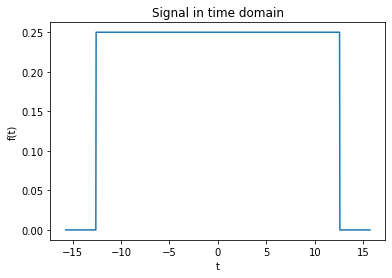
\includegraphics[width=\columnwidth]{signal_time.png}
\caption{Plot of signal in Time domain}
\label{fig:sig_time}
\end{figure}
\begin{figure}[h!]
\centering
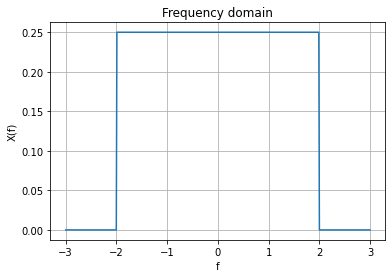
\includegraphics[width=\columnwidth]{signal_freq.png}
\caption{Plot of signal in Frequency domain}
\label{fig:sig_freq}
\end{figure}
\begin{figure}[h!]
\centering
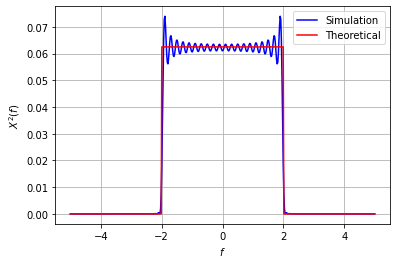
\includegraphics[width=\columnwidth]{signal_freq_squared.png}
\caption{Plot of square of signal in frequency domain}
\label{fig:rect_squared}
\end{figure}
\end{document}
